\chapter{Descriptores}\label{cap_descriptores}
 En este capítulo se detalla el funcionamiento de los descriptores que fueron implementados y probados en la memoria.

\section{Descriptor de Histograma de grises por zona (GHD)}\label{ghd}
El descriptor de histograma de grises o \emph{gray histogram descriptor} busca capturar la distribución espacial de la luz en la imagen usando histogramas de grises~\cite{tesis}. Un histograma de grises, o histograma de intensidad, representa la cantidad de pixeles con cierto rango de intensidad, suponiendo que un pixel tiene intensidad entre 0 y 255 y que el histograma tiene $m$ bins entonces el valor del bin $i$ del histograma representa la cantidad de pixeles en la imagen con intensidad en el intervalo $[\frac{255*i}{m},\frac{255*(i+1)}{m})$.

Para calcular el GHD de una imagen primero se pasa la imagen a escala de grises, luego se divide en $W \times H$ zonas, para cada zona se calcula un histograma de $m$ bins con la intensidad de sus pixeles, para formar el descriptor global de la imagen se concatenan los histogramas de cada zona. La figura~\ref{descriptor_ghd} ilustra el proceso del cálculo del descriptor. El descriptor final es un vector de $W \times H \times m$ dimensiones.
    \begin{figure}[!h]
		\centering
		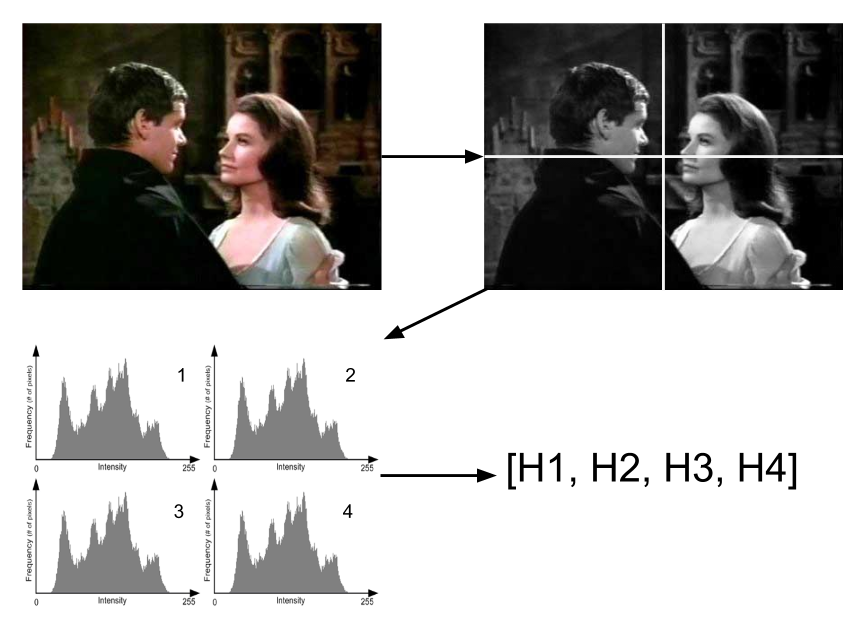
\includegraphics[scale=0.4]{imagenes/cap3/descriptor_ghd.png}
		\caption{Ilustración del algoritmo para calcular el descriptor GHD.}
		\label{descriptor_ghd}
	\end{figure}

\section{Descriptor de distribución de colores (CLD)}\label{cld}
El descriptor de distribución de colores o \emph{color layout descriptor} busca representar la distribución de color en la imagen~\cite{Katsuni:cld, Manjunath:desc}. Para lograr esto se divide en $W \times H$ zonas, para cada zona se calcula el color promedio de sus pixeles, calculando por separado el promedio en cada canal de la imagen RGB, así para cada zona se obtiene tres valores correspondientes a los valores promedio de rojo, verde y azul en la zona. La figura~\ref{descriptor_cld} ilustra el resultado de el proceso anterior.  Se concatenan los resultados de cada zona para formar el descriptor global. El descriptor es un vector de $W \times H \times 3$ dimensiones.
    \begin{figure}[!h]
		\centering
		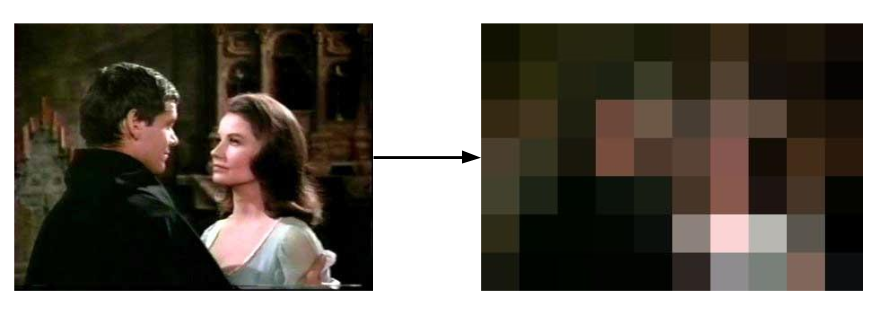
\includegraphics[scale=0.4]{imagenes/cap3/descriptor_kf.png}
		\caption{Ilustración del algoritmo para calcular el descriptor CLD.}
		\label{descriptor_cld}
	\end{figure}

\section{Descriptor de histograma de bordes por zona (EHD)}\label{ehd}
El descriptor de histograma de bordes o \emph{edge histogram descriptor} busca representar la orientación de los bordes presentes en la imagen \cite{ParkJW00:ehd, Manjunath:desc}. Se construye pasando la imagen a escala de grises y particionándola en $W \times H$ zonas, cada zona se subdivide en $M_w \times M_h$ bloques y cada bloque se subdivide en cuatro sub-bloques como muestra la Figura~\ref{ehd_blocks}. De aquí en adelante se trata al sub-bloque como la unidad mínima de la imagen, y su valor corresponde al promedio de intensidad de gris de los pixeles contenidos en el sub-bloque.
    \begin{figure}[!h]
		\centering
		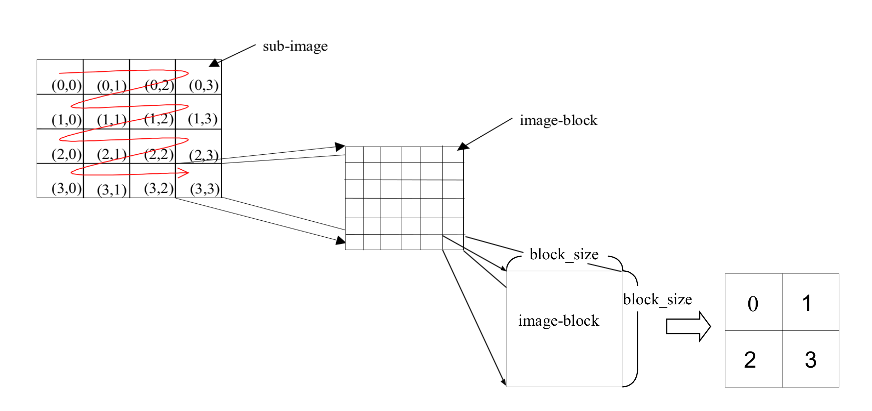
\includegraphics[scale=0.45]{imagenes/cap3/ehd_blocks.png}
		\caption{Subdivision de la imagen usada por el algoritmo del descriptor EHD.}
		\label{ehd_blocks}
	\end{figure}
Cada bloque se clasifica según la orientación de los bordes presentes en él. Se definen cinco tipos de borde ilustrados en la figura~\ref{ehd_blocks}, cada tipo de borde tiene asociado un filtro. Para identificar el tipo de borde presente en un bloque calculamos la \emph{energía} de cada filtro como: 
\begin{equation*}
E_i =  \displaystyle\sum_{i=0}^{1} \left(\displaystyle\sum_{j=0}^{1} \text{filtro}_i(i,j) * \text{subbloque}(i,j)\right)
\end{equation*}

    \begin{figure}[!h]
		\centering
		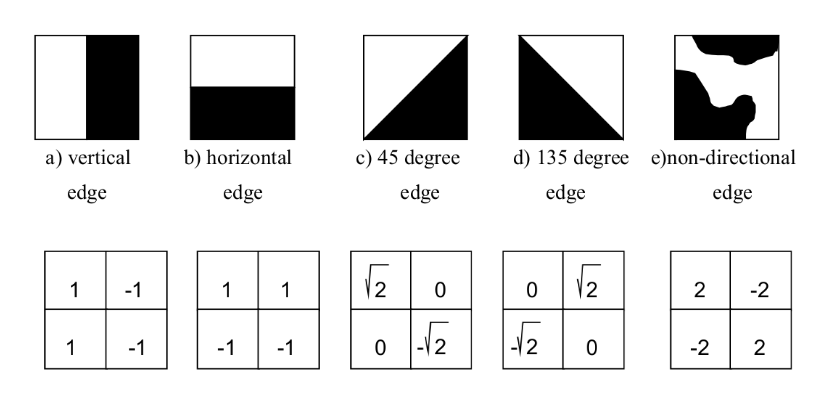
\includegraphics[scale=0.45]{imagenes/cap3/ehd_filters.png}
		\caption{Tipos de borde y sus respectivos filtros para el descriptor EHD.}
		\label{ehd_filters}
	\end{figure}
Para cada bloque calculamos la energía de cada filtro, si el valor de la mayor energía supera un umbral $t$ entonces el bloque se clasifica con el tipo de borde correspondiente, si el mayor no alcanza el valor umbral el bloque se clasifica como sin bordes.

Luego para cada zona se calcula un histograma de cinco bins donde cada bin corresponde a un tipo de borde, y el valor del bin corresponde a la cantidad de bloques dentro de la zona que se clasificaron con ese borde, los bloques clasificados como sin borde no cuentan en el histograma.
Finalmente el descriptor global está dado por la concatenación de los histogramas de cada zona de la imagen. El descriptor final tiene dimensión 
$W \times H \times 5$.

Estos tres tipos de descriptores fueron implementados y comparados en términos de eficacia, es decir, la cantidad de resultados correctos que produjo cada uno al usarlos en la búsqueda. 
